% Options for packages loaded elsewhere
\PassOptionsToPackage{unicode}{hyperref}
\PassOptionsToPackage{hyphens}{url}
%
\documentclass[
]{article}
\usepackage{lmodern}
\usepackage{amssymb,amsmath}
\usepackage{ifxetex,ifluatex}
\ifnum 0\ifxetex 1\fi\ifluatex 1\fi=0 % if pdftex
  \usepackage[T1]{fontenc}
  \usepackage[utf8]{inputenc}
  \usepackage{textcomp} % provide euro and other symbols
\else % if luatex or xetex
  \usepackage{unicode-math}
  \defaultfontfeatures{Scale=MatchLowercase}
  \defaultfontfeatures[\rmfamily]{Ligatures=TeX,Scale=1}
\fi
% Use upquote if available, for straight quotes in verbatim environments
\IfFileExists{upquote.sty}{\usepackage{upquote}}{}
\IfFileExists{microtype.sty}{% use microtype if available
  \usepackage[]{microtype}
  \UseMicrotypeSet[protrusion]{basicmath} % disable protrusion for tt fonts
}{}
\makeatletter
\@ifundefined{KOMAClassName}{% if non-KOMA class
  \IfFileExists{parskip.sty}{%
    \usepackage{parskip}
  }{% else
    \setlength{\parindent}{0pt}
    \setlength{\parskip}{6pt plus 2pt minus 1pt}}
}{% if KOMA class
  \KOMAoptions{parskip=half}}
\makeatother
\usepackage{xcolor}
\IfFileExists{xurl.sty}{\usepackage{xurl}}{} % add URL line breaks if available
\IfFileExists{bookmark.sty}{\usepackage{bookmark}}{\usepackage{hyperref}}
\hypersetup{
  pdftitle={Documentation},
  pdfauthor={Lenka Stastna, Ivana Stanova},
  hidelinks,
  pdfcreator={LaTeX via pandoc}}
\urlstyle{same} % disable monospaced font for URLs
\usepackage[margin=1in]{geometry}
\usepackage{longtable,booktabs}
% Correct order of tables after \paragraph or \subparagraph
\usepackage{etoolbox}
\makeatletter
\patchcmd\longtable{\par}{\if@noskipsec\mbox{}\fi\par}{}{}
\makeatother
% Allow footnotes in longtable head/foot
\IfFileExists{footnotehyper.sty}{\usepackage{footnotehyper}}{\usepackage{footnote}}
\makesavenoteenv{longtable}
\usepackage{graphicx,grffile}
\makeatletter
\def\maxwidth{\ifdim\Gin@nat@width>\linewidth\linewidth\else\Gin@nat@width\fi}
\def\maxheight{\ifdim\Gin@nat@height>\textheight\textheight\else\Gin@nat@height\fi}
\makeatother
% Scale images if necessary, so that they will not overflow the page
% margins by default, and it is still possible to overwrite the defaults
% using explicit options in \includegraphics[width, height, ...]{}
\setkeys{Gin}{width=\maxwidth,height=\maxheight,keepaspectratio}
% Set default figure placement to htbp
\makeatletter
\def\fps@figure{htbp}
\makeatother
\setlength{\emergencystretch}{3em} % prevent overfull lines
\providecommand{\tightlist}{%
  \setlength{\itemsep}{0pt}\setlength{\parskip}{0pt}}
\setcounter{secnumdepth}{5}

\title{Documentation}
\author{Lenka Stastna, Ivana Stanova}
\date{19 11 2020}

\begin{document}
\maketitle

{
\setcounter{tocdepth}{2}
\tableofcontents
}
Nejaký text z čoho pozostavala praca alebo ustredna tema? Zadanie? kto je sponzor? Kroky?

\hypertarget{data-preparation}{%
\section{Data Preparation}\label{data-preparation}}

\hypertarget{data-understanding}{%
\subsection{Data Understanding}\label{data-understanding}}

\hypertarget{data-description-report}{%
\subsubsection{Data Description Report}\label{data-description-report}}

The initial data was provided in a comma-separated values file, and was loaded and processed using the R programming language. Dataset used in this analysis contains 2 353 012 observations and 24 variables. Out of the 24 variables, 13 are of factor datatype, 9 are numeric and 2 are dates.
All columns from the initial data were converted to the correct datype according to the data description file, which was provided. Column \emph{payed\_ammount} was replaced by column \emph{paid\_amount}. Column \emph{payment\_date} originally contained some blank fields, which were subsequently filled in as NA.

\begin{longtable}[]{@{}lll@{}}
\toprule
\begin{minipage}[b]{0.30\columnwidth}\raggedright
Column name\strut
\end{minipage} & \begin{minipage}[b]{0.30\columnwidth}\raggedright
Description\strut
\end{minipage} & \begin{minipage}[b]{0.30\columnwidth}\raggedright
Type\strut
\end{minipage}\tabularnewline
\midrule
\endhead
\begin{minipage}[t]{0.30\columnwidth}\raggedright
contract\_id\strut
\end{minipage} & \begin{minipage}[t]{0.30\columnwidth}\raggedright
Unique identificator of the contract\strut
\end{minipage} & \begin{minipage}[t]{0.30\columnwidth}\raggedright
Int\strut
\end{minipage}\tabularnewline
\begin{minipage}[t]{0.30\columnwidth}\raggedright
payment\_order\strut
\end{minipage} & \begin{minipage}[t]{0.30\columnwidth}\raggedright
Order of the payment\strut
\end{minipage} & \begin{minipage}[t]{0.30\columnwidth}\raggedright
Int\strut
\end{minipage}\tabularnewline
\begin{minipage}[t]{0.30\columnwidth}\raggedright
due\_date\strut
\end{minipage} & \begin{minipage}[t]{0.30\columnwidth}\raggedright
Payment deadline\strut
\end{minipage} & \begin{minipage}[t]{0.30\columnwidth}\raggedright
Date\strut
\end{minipage}\tabularnewline
\begin{minipage}[t]{0.30\columnwidth}\raggedright
payment\_date\strut
\end{minipage} & \begin{minipage}[t]{0.30\columnwidth}\raggedright
Date of the payment\strut
\end{minipage} & \begin{minipage}[t]{0.30\columnwidth}\raggedright
Date\strut
\end{minipage}\tabularnewline
\begin{minipage}[t]{0.30\columnwidth}\raggedright
product\_type\strut
\end{minipage} & \begin{minipage}[t]{0.30\columnwidth}\raggedright
Type of the product\strut
\end{minipage} & \begin{minipage}[t]{0.30\columnwidth}\raggedright
Factor\strut
\end{minipage}\tabularnewline
\begin{minipage}[t]{0.30\columnwidth}\raggedright
contract\_status\strut
\end{minipage} & \begin{minipage}[t]{0.30\columnwidth}\raggedright
Contract status\strut
\end{minipage} & \begin{minipage}[t]{0.30\columnwidth}\raggedright
Factor\strut
\end{minipage}\tabularnewline
\begin{minipage}[t]{0.30\columnwidth}\raggedright
business\_discount\strut
\end{minipage} & \begin{minipage}[t]{0.30\columnwidth}\raggedright
Business discount provided\strut
\end{minipage} & \begin{minipage}[t]{0.30\columnwidth}\raggedright
Factor\strut
\end{minipage}\tabularnewline
\begin{minipage}[t]{0.30\columnwidth}\raggedright
gender\strut
\end{minipage} & \begin{minipage}[t]{0.30\columnwidth}\raggedright
Gender\strut
\end{minipage} & \begin{minipage}[t]{0.30\columnwidth}\raggedright
Factor\strut
\end{minipage}\tabularnewline
\begin{minipage}[t]{0.30\columnwidth}\raggedright
marital\_status\strut
\end{minipage} & \begin{minipage}[t]{0.30\columnwidth}\raggedright
Marital status\strut
\end{minipage} & \begin{minipage}[t]{0.30\columnwidth}\raggedright
Factor\strut
\end{minipage}\tabularnewline
\begin{minipage}[t]{0.30\columnwidth}\raggedright
number\_of\_children\strut
\end{minipage} & \begin{minipage}[t]{0.30\columnwidth}\raggedright
Number of children\strut
\end{minipage} & \begin{minipage}[t]{0.30\columnwidth}\raggedright
Int\strut
\end{minipage}\tabularnewline
\begin{minipage}[t]{0.30\columnwidth}\raggedright
number\_other\_product\strut
\end{minipage} & \begin{minipage}[t]{0.30\columnwidth}\raggedright
Number of other products\strut
\end{minipage} & \begin{minipage}[t]{0.30\columnwidth}\raggedright
Int\strut
\end{minipage}\tabularnewline
\begin{minipage}[t]{0.30\columnwidth}\raggedright
clients\_phone\strut
\end{minipage} & \begin{minipage}[t]{0.30\columnwidth}\raggedright
T/F if the client filled in home phone\strut
\end{minipage} & \begin{minipage}[t]{0.30\columnwidth}\raggedright
Factor\strut
\end{minipage}\tabularnewline
\begin{minipage}[t]{0.30\columnwidth}\raggedright
client\_mobile\strut
\end{minipage} & \begin{minipage}[t]{0.30\columnwidth}\raggedright
T/F if the client filled in mobile phone\strut
\end{minipage} & \begin{minipage}[t]{0.30\columnwidth}\raggedright
Factor\strut
\end{minipage}\tabularnewline
\begin{minipage}[t]{0.30\columnwidth}\raggedright
client\_email\strut
\end{minipage} & \begin{minipage}[t]{0.30\columnwidth}\raggedright
T/F if the client filled in email address\strut
\end{minipage} & \begin{minipage}[t]{0.30\columnwidth}\raggedright
Factor\strut
\end{minipage}\tabularnewline
\begin{minipage}[t]{0.30\columnwidth}\raggedright
total\_earnings\strut
\end{minipage} & \begin{minipage}[t]{0.30\columnwidth}\raggedright
Earning bucket\strut
\end{minipage} & \begin{minipage}[t]{0.30\columnwidth}\raggedright
Factor\strut
\end{minipage}\tabularnewline
\begin{minipage}[t]{0.30\columnwidth}\raggedright
birth\_year\strut
\end{minipage} & \begin{minipage}[t]{0.30\columnwidth}\raggedright
Birth year of the client\strut
\end{minipage} & \begin{minipage}[t]{0.30\columnwidth}\raggedright
Int\strut
\end{minipage}\tabularnewline
\begin{minipage}[t]{0.30\columnwidth}\raggedright
birth\_month\strut
\end{minipage} & \begin{minipage}[t]{0.30\columnwidth}\raggedright
Birth month of the client\strut
\end{minipage} & \begin{minipage}[t]{0.30\columnwidth}\raggedright
Int\strut
\end{minipage}\tabularnewline
\begin{minipage}[t]{0.30\columnwidth}\raggedright
living\_area\strut
\end{minipage} & \begin{minipage}[t]{0.30\columnwidth}\raggedright
Region of the client home address\strut
\end{minipage} & \begin{minipage}[t]{0.30\columnwidth}\raggedright
Factor\strut
\end{minipage}\tabularnewline
\begin{minipage}[t]{0.30\columnwidth}\raggedright
different\_contact\_area\strut
\end{minipage} & \begin{minipage}[t]{0.30\columnwidth}\raggedright
T/F if the client filled different home and contact address\strut
\end{minipage} & \begin{minipage}[t]{0.30\columnwidth}\raggedright
Factor\strut
\end{minipage}\tabularnewline
\begin{minipage}[t]{0.30\columnwidth}\raggedright
kc\_flag\strut
\end{minipage} & \begin{minipage}[t]{0.30\columnwidth}\raggedright
T/F if the client does not home local citizenship\strut
\end{minipage} & \begin{minipage}[t]{0.30\columnwidth}\raggedright
Factor\strut
\end{minipage}\tabularnewline
\begin{minipage}[t]{0.30\columnwidth}\raggedright
cf\_val\strut
\end{minipage} & \begin{minipage}[t]{0.30\columnwidth}\raggedright
If the special measure during the underwriting was applied\strut
\end{minipage} & \begin{minipage}[t]{0.30\columnwidth}\raggedright
\strut
\end{minipage}\tabularnewline
\begin{minipage}[t]{0.30\columnwidth}\raggedright
kzmz\_flag\strut
\end{minipage} & \begin{minipage}[t]{0.30\columnwidth}\raggedright
T/F if the client filled in employer\strut
\end{minipage} & \begin{minipage}[t]{0.30\columnwidth}\raggedright
Factor\strut
\end{minipage}\tabularnewline
\begin{minipage}[t]{0.30\columnwidth}\raggedright
due\_amount\strut
\end{minipage} & \begin{minipage}[t]{0.30\columnwidth}\raggedright
Installment what should be payed\strut
\end{minipage} & \begin{minipage}[t]{0.30\columnwidth}\raggedright
Numeric\strut
\end{minipage}\tabularnewline
\begin{minipage}[t]{0.30\columnwidth}\raggedright
payed\_amount\strut
\end{minipage} & \begin{minipage}[t]{0.30\columnwidth}\raggedright
What was payed at a certain date\strut
\end{minipage} & \begin{minipage}[t]{0.30\columnwidth}\raggedright
Numeric\strut
\end{minipage}\tabularnewline
\bottomrule
\end{longtable}

\hypertarget{value-ranges}{%
\subsubsection{Value ranges}\label{value-ranges}}

Frequency, relative frequency and relative cumulative frequency were computed for each category in all categorical variables. All frequency tables can be located in the ``frequencies'' list.

\hypertarget{attribute-correlations}{%
\subsubsection{Attribute correlations}\label{attribute-correlations}}

\begin{figure}
\centering
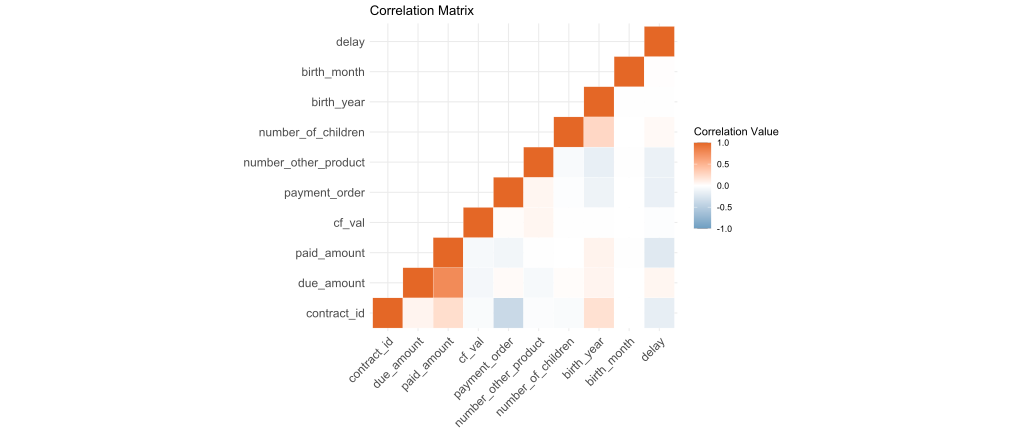
\includegraphics{Correlogram.svg}
\caption{correlogram}
\end{figure}

We computed correlation coefficients between all possible pairs of numeric variables, see Figure \ref{fig:correlogram}, and discovered strong positive correlation between due amount and paid amount. This could be due to the fact that in the event that the installment has already been paid, the due amount and the paid amount would assume the same value. Correlation between the remaining pairs of numeric variables was either nonexistent or negligible.
Then, the significance of correlation between due amount and paid amount was tested using Pearson's product moment correlation coefficient. The pair of attributes was found to be significantly correlated with a correlation coefficient of 0.76 and p-value less than 2.2e-16.

Relationship between categorical variables was tested using chi-squared test with the significance level of 0.05. All significantly correlated pairs of variables can be accessed in ``categorical\_rel'' dataframe.

\hypertarget{basic-statistics}{%
\paragraph{Basic statistics}\label{basic-statistics}}

Basic statistics computed for numeric variables can be located in Table @ref\{tab:statistics\}. Distribution of numeric and categorical variables was visualized using boxplots, density plots and histograms, see in Attachments, Figure \ref{fig:boxplots} and Figure \ref{fig:density}.

\hypertarget{data-exploration-report}{%
\subsection{Data Exploration Report}\label{data-exploration-report}}

NIECO HODIT

\hypertarget{data-quality-report}{%
\subsection{Data Quality Report}\label{data-quality-report}}

\hypertarget{data-coverage}{%
\subsubsection{Data coverage}\label{data-coverage}}

Next step consited of the data coverage analysis. As an example, we have chosen a couple of plots, that indicate interesting data distribution.
We for example found out, that clients mostly order the product type 1, contracts are mostly in status number 1 or that most of the payments have a discount.
We also discovered, that the marital status of the clients is mostly number 3 and they have most frequently no children. Clients also very frequently do not provide information about their earnings and they ordered usually 1 other product.

All the mentioned findings can be seen on visualizations on Figure \ref{fig:distribution}. All the data coverage visualizations are available in the Attachments.

\includegraphics{Documentation_Rmarkdown_files/figure-latex/distribution-1.pdf}

\hypertarget{missing-values}{%
\subsubsection{Missing values}\label{missing-values}}

Exploring the NA values in the dataset, we found out, that 4 attributes had
almost same percentage of missing values, as can be seen on the statistics on Figure @ref(fig:Missing\_stat).
Attributes kc\_flag, living\_area, cf\_val and different\_contact\_area have the most missing values, almost 20 \%, whereas payment\_order has around 3,5 \% and payment\_date and delay have the same percentage, almost 0,5 \%.

Using a different visualization, that can be seen on Figure @ref(fig:Missing\_complex),
we discovered, that the four attributes with the highest percentage are
not missing at random but almost all at the same time.

We found out, that contract\_id together with payment\_order were not creating a unique key of the data payment,
but one payment was divided into multiple parts, which was also causing problem with NA values in the four attributes. Data in the four attributes were not copied into other parts of a payment, but were present in just the first payment part.
We decided to unify the payment parts into only one payment by summarizing the
paid amount of all the parts and using the payment\_date of the last paid part.
Thanks to the unification, the amount of NA values has markedly decreased.

Secondly, we dealt with the NA values in payment\_order and payment\_date.
Since it was only less then 4 \% of the dataset, and it was not possible to
substitute the values, we decided to delete the rows.

\begin{verbatim}
## # A tibble: 25 x 3
##    variable               n_miss pct_miss
##    <chr>                   <int>    <dbl>
##  1 different_contact_area 471354   20.0  
##  2 cf_val                 469310   19.9  
##  3 living_area            469015   19.9  
##  4 kc_flag                468906   19.9  
##  5 payment_order           83361    3.54 
##  6 payment_date            11733    0.499
##  7 delay                   11733    0.499
##  8 contract_id                 0    0    
##  9 due_date                    0    0    
## 10 product_type                0    0    
## # ... with 15 more rows
\end{verbatim}

\begin{figure}
\centering
\includegraphics{Documentation_Rmarkdown_files/figure-latex/Missing_complex-1.pdf}
\caption{(\#fig:Missing\_complex)\label{fig:Missing_complex}Distribution of missing values}
\end{figure}

\begin{figure}
\centering
\includegraphics{missing_values_plot.png}
\caption{missing\_values\_plot}
\end{figure}

\hypertarget{feature-engineering}{%
\subsection{Feature engineering}\label{feature-engineering}}

We decided to add new features to create higher-accuracy models.
First of all, we computed a numerical feature ``delay'' counting the difference between payment\_date and due\_date.

Since we are creating two classification models deciding whether a new payment will be delayed
for more than 21 days or more than 140 days, we created 2 new binary features ``delay\_21\_y'' and ``delay\_140\_y''.

We also created a new numerical feature ``delay\_indiv'' counting the mean delay for the whole client´s history. We also computed 2 new numerical features, ``delay\_indiv\_21'' and ``delay\_indiv\_140'' counting cumulative number of delayed payments (21, 140 days) by one contract

Lastly, numerical features ``mean\_delay\_1m'' ,``mean\_delay\_3m'', ``mean\_delay\_6m'', ``mean\_delay\_12m'' are computing the mean delay for 1/3/6/12 months for each contract.

\hypertarget{exploratory-analysis-of-the-new-features}{%
\subsection{Exploratory analysis of the new features}\label{exploratory-analysis-of-the-new-features}}

\hypertarget{data-description-report-1}{%
\subsubsection{Data description report}\label{data-description-report-1}}

\begin{longtable}[]{@{}lll@{}}
\toprule
\begin{minipage}[b]{0.30\columnwidth}\raggedright
Column name\strut
\end{minipage} & \begin{minipage}[b]{0.30\columnwidth}\raggedright
Description\strut
\end{minipage} & \begin{minipage}[b]{0.30\columnwidth}\raggedright
Type\strut
\end{minipage}\tabularnewline
\midrule
\endhead
\begin{minipage}[t]{0.30\columnwidth}\raggedright
delay\strut
\end{minipage} & \begin{minipage}[t]{0.30\columnwidth}\raggedright
Difference between payment\_date and due\_date\strut
\end{minipage} & \begin{minipage}[t]{0.30\columnwidth}\raggedright
Int\strut
\end{minipage}\tabularnewline
\begin{minipage}[t]{0.30\columnwidth}\raggedright
delay\_21\_y\strut
\end{minipage} & \begin{minipage}[t]{0.30\columnwidth}\raggedright
T/F if the delay is more than 21 days\strut
\end{minipage} & \begin{minipage}[t]{0.30\columnwidth}\raggedright
Factor\strut
\end{minipage}\tabularnewline
\begin{minipage}[t]{0.30\columnwidth}\raggedright
delay\_140\_y\strut
\end{minipage} & \begin{minipage}[t]{0.30\columnwidth}\raggedright
T/F if the delay is more than 140 days\strut
\end{minipage} & \begin{minipage}[t]{0.30\columnwidth}\raggedright
Int\strut
\end{minipage}\tabularnewline
\begin{minipage}[t]{0.30\columnwidth}\raggedright
delay\_indiv\strut
\end{minipage} & \begin{minipage}[t]{0.30\columnwidth}\raggedright
Mean delay for the whole client's history\strut
\end{minipage} & \begin{minipage}[t]{0.30\columnwidth}\raggedright
Int\strut
\end{minipage}\tabularnewline
\begin{minipage}[t]{0.30\columnwidth}\raggedright
delay\_indiv\_21\strut
\end{minipage} & \begin{minipage}[t]{0.30\columnwidth}\raggedright
Cumulative sum of payments delayed for more than 21 days by contract\strut
\end{minipage} & \begin{minipage}[t]{0.30\columnwidth}\raggedright
Int\strut
\end{minipage}\tabularnewline
\begin{minipage}[t]{0.30\columnwidth}\raggedright
delay\_indiv\_140\strut
\end{minipage} & \begin{minipage}[t]{0.30\columnwidth}\raggedright
Cumulative sum of the payments delayed for more than 140 days by contract\strut
\end{minipage} & \begin{minipage}[t]{0.30\columnwidth}\raggedright
Int\strut
\end{minipage}\tabularnewline
\begin{minipage}[t]{0.30\columnwidth}\raggedright
mean\_delay\_1m\strut
\end{minipage} & \begin{minipage}[t]{0.30\columnwidth}\raggedright
Average payment delay for the last month\strut
\end{minipage} & \begin{minipage}[t]{0.30\columnwidth}\raggedright
Int\strut
\end{minipage}\tabularnewline
\begin{minipage}[t]{0.30\columnwidth}\raggedright
mean\_delay\_3m\strut
\end{minipage} & \begin{minipage}[t]{0.30\columnwidth}\raggedright
Average payment delay for the last 3 months\strut
\end{minipage} & \begin{minipage}[t]{0.30\columnwidth}\raggedright
Int\strut
\end{minipage}\tabularnewline
\begin{minipage}[t]{0.30\columnwidth}\raggedright
mean\_delay\_6m\strut
\end{minipage} & \begin{minipage}[t]{0.30\columnwidth}\raggedright
Average payment delay for the last 6 months\strut
\end{minipage} & \begin{minipage}[t]{0.30\columnwidth}\raggedright
Int\strut
\end{minipage}\tabularnewline
\begin{minipage}[t]{0.30\columnwidth}\raggedright
mean\_delay\_12m\strut
\end{minipage} & \begin{minipage}[t]{0.30\columnwidth}\raggedright
Average payment delay for the last 12 months\strut
\end{minipage} & \begin{minipage}[t]{0.30\columnwidth}\raggedright
Int\strut
\end{minipage}\tabularnewline
\bottomrule
\end{longtable}

\hypertarget{basic-statistics-1}{%
\subsubsection{Basic statistics}\label{basic-statistics-1}}

We computed basic statistics for each new attribute.
All the visualizations can be seen on @ref(fig:stat\_new\_delay).

First of all we focused on attribute delay. Since it is probably the most important attribute of the nexly created, we analysed its distribution, distribution of delay on log scale DOPLNIT CO SME NASLI.
\includegraphics{Documentation_Rmarkdown_files/figure-latex/stat_new_delay-1.pdf}

\begin{verbatim}
## [[1]]
\end{verbatim}

\begin{figure}
\centering
\includegraphics{Documentation_Rmarkdown_files/figure-latex/stat_new_delay-2.pdf}
\caption{(\#fig:stat\_new\_delay-2)\label{fig:stat_new_delay}Basic statistics of the added attribute delay.}
\end{figure}

\begin{verbatim}
## 
## [[2]]
## NULL
## 
## [[3]]
\end{verbatim}

\begin{figure}
\centering
\includegraphics{Documentation_Rmarkdown_files/figure-latex/stat_new_delay-3.pdf}
\caption{(\#fig:stat\_new\_delay-3)\label{fig:stat_new_delay}Basic statistics of the added attribute delay.}
\end{figure}

\begin{verbatim}
## 
## [[4]]
\end{verbatim}

\includegraphics{Documentation_Rmarkdown_files/figure-latex/stat_new_delay-4.pdf}
\includegraphics{delay_boxplot.png}
We also computed some basic statistics for the other added attributes. DOPLNIT CO SME NASLI
\includegraphics{Documentation_Rmarkdown_files/figure-latex/stat_new-1.pdf}

\hypertarget{missing-values-1}{%
\subsubsection{Missing values}\label{missing-values-1}}

As can be seen on Figure, newly-created features also contain NA values. The highest percentage of missing values has attribute mean\_delay\_12m, almost 55 \%. Together with mean\_delay\_6m, mean\_delay\_3m and mean\_delay\_1m, they are the only new attributes holding NA attributes.

It is not surprising, that these attributes have the highest percentage of NAs, since they compute results only every 12/6/3/1 months.

We decided to replace the NA values by 0, so they can be later used in the modeling part.

\begin{verbatim}
## # A tibble: 34 x 3
##    variable               n_miss pct_miss
##    <chr>                   <int>    <dbl>
##  1 mean_delay_12m         804268    55.4 
##  2 mean_delay_6m          458935    31.6 
##  3 mean_delay_3m          249422    17.2 
##  4 mean_delay_1m           95489     6.58
##  5 contract_id                 0     0   
##  6 payment_order               0     0   
##  7 due_date                    0     0   
##  8 living_area                 0     0   
##  9 different_contact_area      0     0   
## 10 kc_flag                     0     0   
## # ... with 24 more rows
\end{verbatim}

\hypertarget{advanced-statistics}{%
\subsection{Advanced statistics}\label{advanced-statistics}}

\includegraphics{Dependence of paid amount on gender, product type and business discount.svg}
\includegraphics{Distribution of due amount by contract status.png}
\includegraphics{Distribution of paid amount according to total earnings.png}
\includegraphics{Paid amount by product type.png}
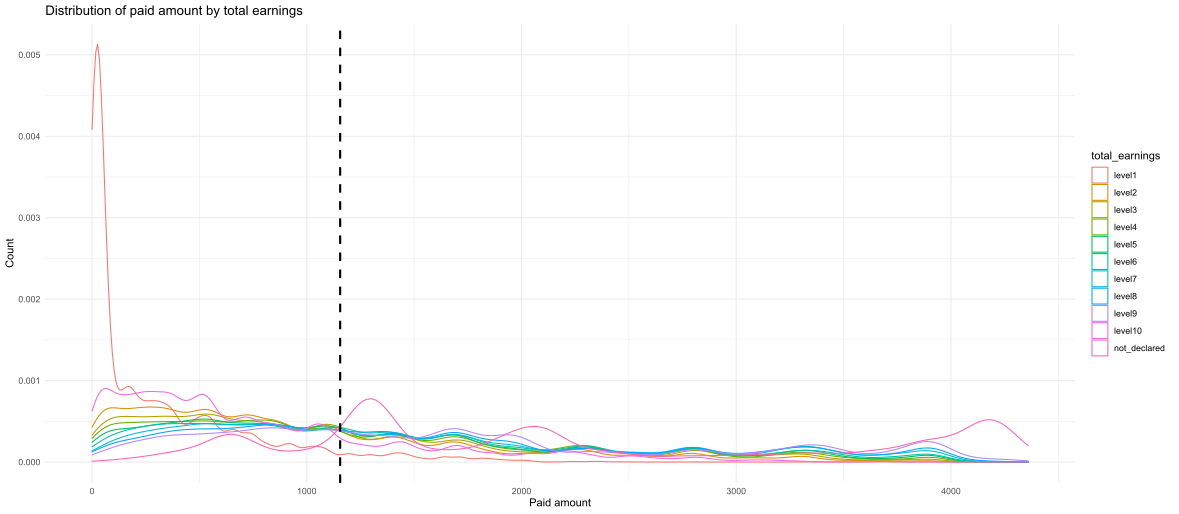
\includegraphics{Paid amount by total earnings.png}

\includegraphics{Statistical dependence of delay on gender.png}
\includegraphics{Statistical dependence of due amount on gender.png}
\includegraphics{Statistical dependence of paid amount on gender, product type and business discount.png}
\includegraphics{Statistical dependence of paid amount on gender.png}

\hypertarget{modeling}{%
\section{Modeling}\label{modeling}}

\hypertarget{prediction-model-21-days}{%
\subsection{Prediction model (21+ days)}\label{prediction-model-21-days}}

\hypertarget{prediction-model-140-days}{%
\subsection{Prediction model (140+ days)}\label{prediction-model-140-days}}

\hypertarget{estimation-of-the-expected-number-of-days-of-delay-when-the-client-triggers-first-action}{%
\subsection{Estimation of the expected number of days of delay when the client triggers first action}\label{estimation-of-the-expected-number-of-days-of-delay-when-the-client-triggers-first-action}}

\hypertarget{conclusion}{%
\section{Conclusion}\label{conclusion}}

\hypertarget{discussion}{%
\section{Discussion}\label{discussion}}

\hypertarget{attachments}{%
\section{Attachments}\label{attachments}}

\begin{figure}
\centering
\includegraphics{Documentation_Rmarkdown_files/figure-latex/density-1.pdf}
\caption{\label{fig:density}\label{fig:density}Density plots.}
\end{figure}

\begin{figure}
\centering
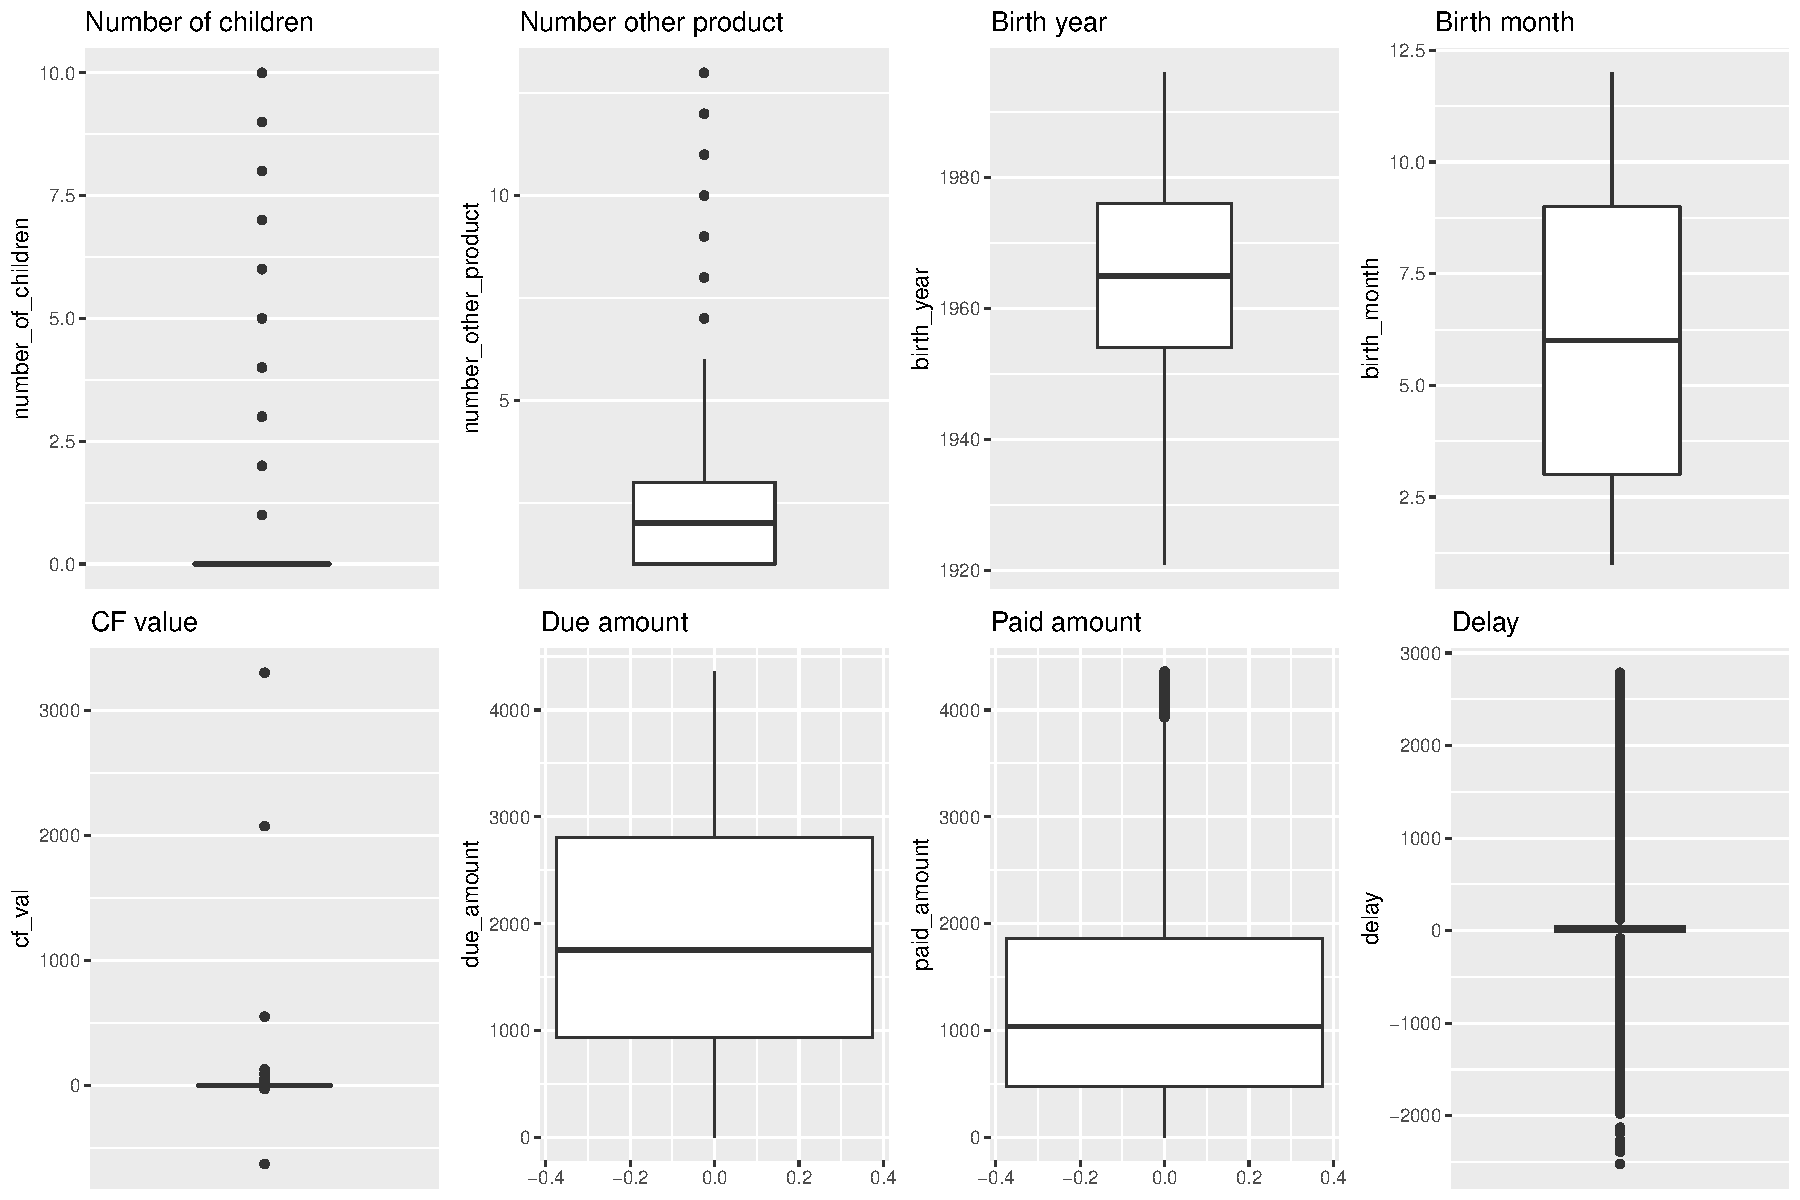
\includegraphics{Documentation_Rmarkdown_files/figure-latex/boxplots-1.pdf}
\caption{\label{fig:boxplots}\label{fig:boxplots}Boxplots for numeric attributes.}
\end{figure}

\end{document}
